\documentclass[twocolumn,10pt]{article}

\usepackage[utf8]{inputenc}
\usepackage[T1]{fontenc}
\usepackage[british]{babel}

\usepackage{lmodern}
\usepackage[sc]{mathpazo} % or option osf
\usepackage{newpxmath}

\usepackage{amsmath}
\usepackage{graphicx}

\usepackage{adjustbox}
\usepackage[a4paper, margin=1mm, includefoot, footskip=15pt]{geometry}

\usepackage[pdftitle={Estimating stem tapper shape by using tree diameter,
 height and volume}
, pdfauthor={Georg Kindermann}
, pdfsubject={stem tapper shape of a tree}
, pdfkeywords={Foresty, stem shape, forest measuration, stem tapper curve}
, pdflang={en-GB}
, colorlinks=true
, linkcolor=blue
, urlcolor=blue
, pdfpagemode=UseNone]{hyperref}

\nonfrenchspacing
\sloppy

\title{Estimating stem tapper shape by using tree diameter, height and volume}
\author{Georg Kindermann}
%\date{10. October 2023}

\begin{document}

\maketitle

%\begin{abstract}
%  Statistik mit Julia.
%\end{abstract}

%\tableofcontents

%\section{Einleitung}
%\label{sec:einleitung}

When measuring trees, typical their diameter (DBH - diameter at breast height in
1.3\,m height above ground) is measured. Nowadays more and more also the height
of each single tree is measured. Alternatively the height is calculated by using
a relation between DBH and height. The volume is calculated by using DBH and
height and a form factor. The form factor could also be estimated by using BHD
and height. Sometimes additional diameters, at different heights on the tree,
are measured to estimate the stem volume and the shape of the tapper. The tapper
shape can be used to split up the stem and its volume into different diameter
classes called assortments.

Calculating the stem volume by using species, DBH and height is a standard task
which was done in the past by using precalculated tables and is done now
typically by using functions. Getting the assortments could also be done by
using functions but is still done by using precalculated tables, as the
functions, for getting the shape and the algorithm of cutting the tree into logs
is somehow complex.

Here I will show a method which is using $d_x = c_0 \cdot (h - x)^{c_1}$, one of
the simplest equation to describe the tapper shape. $d_x$ is the stem diameter
at height $x$, $h$ is the total height of the tree, $x$ is the height
from the ground where the diameter $d_x$ should be estimated and $c_0$ and
$c_1$ are tree specific coefficients.

Instead of the diameter $d_x$ also the crosscutting area $g_x$ could be
estimated with the same equation $g_x = c_2 \cdot (h - x)^{c_3}$ but with
different coefficients. While $g_x = d^2_x \cdot \pi / 4$ follows that $c_3 = 2
\cdot c_1$ and $c_2 = c^2_0 * \pi / 4$.

The integral of the crosscutting area along the stem is the stem volume $V$:
$$V =
\int_{x=0}^h c_2 \cdot (h - x)^{c_3} dx = \frac{c_2
\cdot h^{(c_3 + 1)}}{c_3 + 1}$$

With those relations it's possible to get $c_0$ and $c_1$ for a tree where DBH,
height and volume is known.
\begin{eqnarray*}
g_{1.3} & = & (\text{BHD}/2)^2\pi\\
c_3 & = & \frac{W_0\left(\frac{g_{1.3}*(h-1.3)*log(1-1.3/h)}{V}\right)}{log(1 - 1.3/h)} - 1\\
g_0 & = & g_{1.3} / (1-1.3/h)^{c_3}\\
c_2 & = & g_0 / h^{c_3}\\
g_x & = & c_2 \cdot (h - x)^{c_3}\\
g_x & = & g_0 \cdot (1 - x/h)^{c_3}
\end{eqnarray*}

Where all tree dimensions (DBH, h, V) are in m and m$^3$,
and $W_0()$ is Lamberts W function: $w = W(we^w)$.

When splitting the stem at the height of the DBH into two parts, and it is
assumed that the lower part has the shape of a cylinder, the coefficient can be
estimated with:
\begin{eqnarray*}
V_{>1.3} & = & V - g_{1.3} * 1.3\\
c_5 & = & \frac{g_{1.3} \cdot (h - 1.3)}{V_{>1.3}} - 1\\
c_4 & = & g_{1.3} / (h-1.3)^{c_5}\\
g_x & = & \begin{cases}
    c_4 \cdot (h - x)^{c_5} & \text{if } x\geq 1.3m\\
    g_{1.3}               & \text{otherwise}
    \end{cases}
\end{eqnarray*}

It is also possible to make an assumption of the stem diameter at height 0, like
that it is 1.3\,cm larger than the DBH for trees higher than 1.3\,m and for
smaller trees the diameter is the height / 100. In this case there is no need that the tapper shape goes through the DBH.
\begin{eqnarray*}
d_{0a} & = & \begin{cases}
    DBH + 0.013 & \text{if } h\geq 1.3m\\
    h / 100     & \text{otherwise}
    \end{cases}\\
g_{0a} & = & (d_{0a}/2)^2*pi\\
c_7 & = & \frac{g_{0a} \cdot h}{V} - 1\\
c_6 & = & g_{0a} / h^{c_7}\\
g_x & = & c_6 \cdot (h - x)^{c_7}\\
\end{eqnarray*}

Note that all three shown methods to estimate $g_x$ can give for a specific
height different values. All give monotonic decreasing or steady diameters from
the ground up to the treetop and all come to the same stem volume. It can be
used for diameter and volume with or without bark.

\par\noindent\rule{\columnwidth}{0.5pt}
\par\noindent\rule{\columnwidth}{0.5pt}

For a practical example assume a tree with the following dimensions.
\begin{verbatim}
DBH = 0.252 m
h = 27.5 m
\end{verbatim}

The diameter of the stem was measured at height 0.5\,m, 1.5\,m, 2.5\,m, \dots,
26.5\,m and is given in m (see fig.~\ref{fig:trunk}):
\begin{verbatim}
.261, .250, .242, .245, .237, .228, .220, .218, .213,
.206, .203, .197, .190, .182, .176, .165, .157, .149,
.140, .126, .116, .112, .092, .082, .063, .046, .026
\end{verbatim}

According to Huber the stem volume can be calculated with:
$$V = \sum l \cdot d^2l\pi/4 = 1(0.261^2 + 0.250^ + ... + 0.026^2)\pi/4 = 0.6902m^3$$

\par\noindent\rule{\columnwidth}{0.5pt}

The basal area at breast height is:
$$ g_{1.3} = \text{BHD}^2pi/4 = 0.252^2\pi/4 = 0.04988m^2$$

And the coefficient $c_3$ is calculated with:
\begin{eqnarray*}
c_3 & = & \frac{W_0\left(\frac{g_{1.3}*(h-1.3)*log(1-1.3/h)}{V}\right)}{log(1 - 1.3/h)} - 1\\
 & = & \frac{W_0\left(\frac{0.04988*(27.5-1.3)*log(1-1.3/27.5)}{0.6902}\right)}{log(1 - 1.3/27.5)} - 1\\
  & = & 1.09545
\end{eqnarray*}

And the coefficient $c_2$ is calculated with:
\begin{eqnarray*}
g_0 & = & g_{1.3} / (1-1.3/h)^{c_3}\\
 & = & 0.04988 / (1-1.3/27.5)^{1.09545}\\
 & = & 0.05259m^2 \\
c_2 & = & g_0 / h^{c_3}\\
 & = & 0.05259 / 27.5^{1.09545}\\
 & = & 0.001394
\end{eqnarray*}

And the coefficient $c_0$ and $c_1$ are calculated with:
\begin{eqnarray*}
c_0 & = & \sqrt{c_2 4 / \pi} = \sqrt{0.001394 \cdot 4 / \pi} = 0.04213\\
c_1 & = & c_3/2 = 1.09545/2 = 0.5477
\end{eqnarray*}

The Volume would be:
\begin{eqnarray*}
V & = & \frac{c_2 \cdot h^{(c_3 + 1)}}{c_3 + 1} =
  \frac{0.001394 \cdot 27.5^{(1.09545 + 1)}}{1.09545 + 1} = 0.6902m^3
\end{eqnarray*}

And the diameter at height $x$ is:
\begin{eqnarray*}
d_x & = & c_0 \cdot (h - x)^{c_1} = 0.04213 \cdot (27.5 - x)^{0.5477}\\
d_{1.3} & = & 0.04213 \cdot (27.5 - 1.3)^{0.5477} = 0.252m\\
\end{eqnarray*}

The pattern is shown in fig.~\ref{fig:trunk} as "through DBH".

\par\noindent\rule{\columnwidth}{0.5pt}

Assuming the stem is a cylinder below the DBH the calculation will be:

\begin{eqnarray*}
V_{>1.3} & = & V - g_{1.3} * 1.3 = 0.6902 - 0.04988 * 1.3 = 0.6254\\
c_5 & = & \frac{g_{1.3} \cdot (h - 1.3)}{V_{>1.3}} - 1\\
  & = & \frac{0.04988 \cdot (27.5 - 1.3)}{0.6254} - 1\\
  & = & 1.0895\\
c_4 & = & g_{1.3} / (h-1.3)^{c_5} = 0.04988 / (27.5-1.3)^{1.0895} = 0.001421\\
V & = & \frac{c_4 \cdot (h-1.3)^{(c_5 + 1)}}{c_5 + 1} + g_{1.3} * 1.3\\
 & = & \frac{0.001421 \cdot h^{(1.0895 + 1)}}{1.0895 + 1} + 0.04988 * 1.3\\
 & = & 0.6902m^3\\
g_x & = & \begin{cases}
    c_4 \cdot (h - x)^{c_5} = 0.001421 \cdot (27.5 - x)^{1.0895} & \text{if } x\geq 1.3m\\
    g_{1.3} = 0.04988              & \text{otherwise}
    \end{cases}\\
d_{1.3} & = & \sqrt{c_4 \cdot (h - 1.3)^{c_5} \cdot 4/\pi}\\
 & = & \sqrt{0.001421 \cdot (27.5 - 1.3)^{1.0895} \cdot 4/\pi}\\
 & = & 0.252m
\end{eqnarray*}

The pattern is shown in fig.~\ref{fig:trunk} as "Cylinder".

\par\noindent\rule{\columnwidth}{0.5pt}

Assuming diameter on the ground is 0.013\,m larger than the DBH the calculation
will be:
\begin{eqnarray*}
d_{0a} & = & DBH + 0.013 = 0.252 + 0.013 = 0.265m\\
g_{0a} & = & (d_{0a}/2)^2\pi = (0.265/2)^2\pi = 0.05515m^2\\
c_7 & = & \frac{g_{0a} \cdot h}{V} - 1 = \frac{0.05515 \cdot 27.5}{0.6902} - 1 = 1.1975\\
c_6 & = & g_{0a} / h^{c_7} = 0.05515 / 27.5^{1.1975} = 0.001042\\
V & = & \frac{c_6 \cdot h^{(c_7 + 1)}}{c_7 + 1} = 
\frac{0.001042 \cdot 27.5^{(1.1975 + 1)}}{1.1975 + 1} = 0.6902m^3\\
g_x & = & c_6 \cdot (h - x)^{c_7} = 0.001042 \cdot (h - x)^{1.1975}\\
d_0 & = & = \sqrt{0.001042 \cdot (h - 0)^{1.1975} \cdot 4/\pi} = 0.265m\\
\end{eqnarray*}

The pattern is shown in fig.~\ref{fig:trunk} as "through DBH+1.3".

\begin{figure}[htb]
    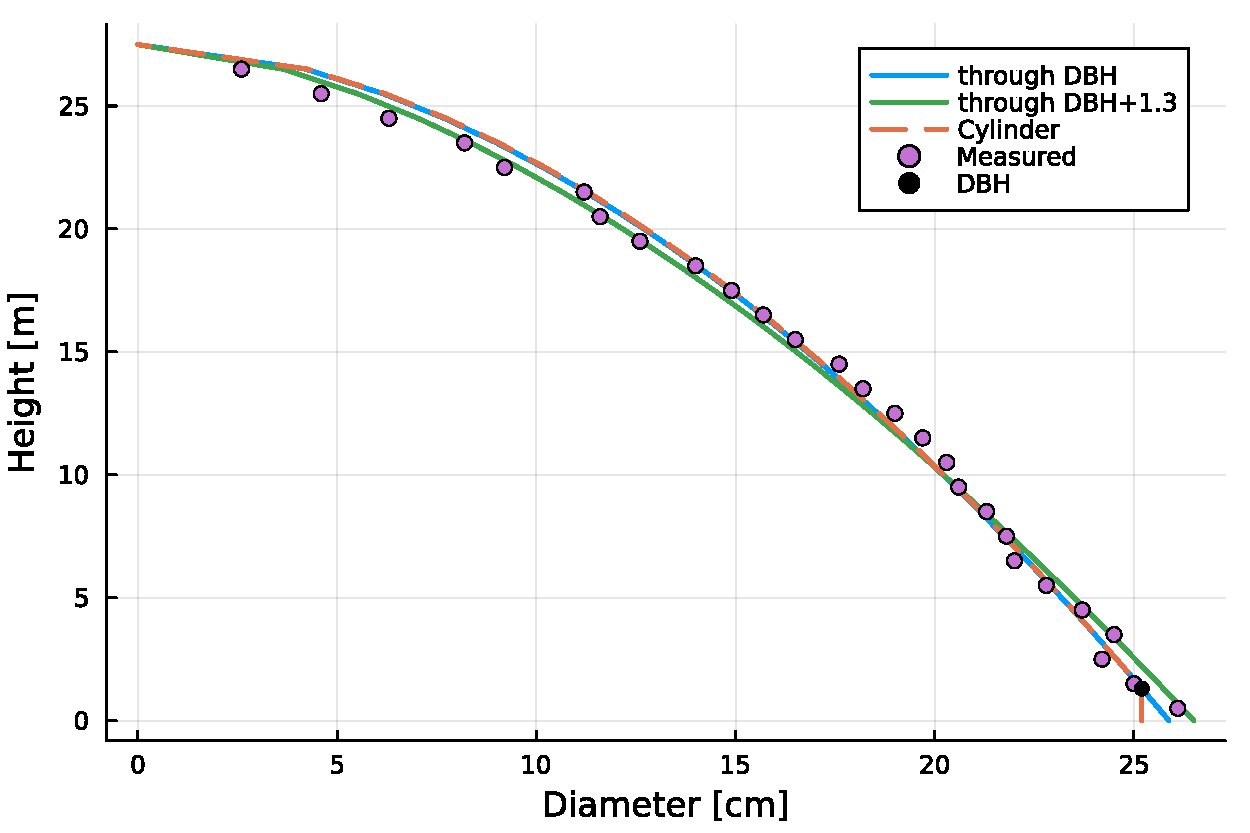
\includegraphics[width=\columnwidth]{trunk}
    \caption{Different methods to estimate tapper curve}
    \label{fig:trunk}
\end{figure}




%Autor: Georg Kindermann

\end{document}